\section{Author Concentration}

Similar to as we saw in Section \ref{subreddit vector}, for each author $a_i$ there are $n$ number of subreddits they commented in. For the $nth$ subreddit author $a_i$ there are $x_n$ number of comments, such that for each author we have the vector:

$$a_i = [x_1, x_2, \cdots x_n]$$

I then use this vector to calculate the three diversity measures as described in Sections \ref{entropy}, \ref{blau index}, and \ref{gini}. For each author we have the following measures:

\begin{itemize}
    \item number of subreddits
    \item number of comments
    \item author comment entropy
    \item author comment gini
    \item author comment blau
\end{itemize}


\subsection{Author In-subreddit Ratio}
I also calculate the author in-subreddit ratio for each author, for each subreddit they commented in.
For author $A$ and subreddit $S$, if $x_S$ is the number of comments $A$ made in $S$ and $\sum A_i$ is the number of comments $A$ made across all subreddits, the author in-subreddit ratio is:

$$insub_A{}_S = \frac{x_s}{\sum A_i}$$

\subsection{Aggregating to Subreddit Level}
Section \ref{sub diversity} characterised subreddits by how authors behaved within subreddits. By now focusing on author activity across subreddits, we can look at how subreddits consists of authors who actor outside of their own space...

By aggregating author statistics to the subreddit level we can determine in certain subreddits tend to attract/consist of authors who are more or less diverse across the entire Reddit platform. For each subreddit I take the median value of each value across all authors who commented in that subreddit. For example, if 500 authors commented in r/ExampleSubreddit, I would take the median value of comment entropy for those 500 authors. I then repeat this for all variables, for all subreddits.

% Author-Level Figure
\begin{table}
\centering
\begin{tabular}{lrrrrrr}
\toprule
{} &  aut\_sub\_count &  aut\_com\_count &  aut\_com\_entropy &  aut\_com\_gini &  aut\_com\_blau &     aut\_insub \\
\midrule
mean &     213.520226 &   5.411813e+03 &         1.645732 &     -1.954438 &      0.597107 &  2.619530e-01 \\
std  &     915.413325 &   7.113781e+04 &         1.452357 &      0.476181 &      0.301553 &  3.383600e-01 \\
min  &       1.000000 &   1.000000e+00 &         0.000000 &     -3.000000 &      0.000000 &  8.030606e-07 \\
25\%  &       3.000000 &   6.000000e+00 &         0.693147 &     -2.018923 &      0.463138 &  2.941176e-02 \\
50\%  &       6.500000 &   1.950000e+01 &         1.428056 &     -1.788352 &      0.687500 &  9.638554e-02 \\
75\%  &      14.500000 &   5.800000e+01 &         2.086235 &     -1.650794 &      0.820000 &  3.333333e-01 \\
max  &    7996.000000 &   1.245236e+06 &         7.672562 &     -1.089127 &      0.998361 &  1.000000e+00 \\
\bottomrule
\end{tabular}
\caption{Distribution of Author Medians for All Subreddits}
\label{table/author-medians:all}
\end{table}
\begin{table}
\centering
\begin{tabular}{lrrrrrr}
\toprule
{} &  aut\_sub\_count &  aut\_com\_count &  aut\_com\_entropy &  aut\_com\_gini &  aut\_com\_blau &  aut\_insub \\
\midrule
mean &          8.180 &         25.049 &            1.530 &        -1.785 &         0.693 &      0.163 \\
std  &          5.122 &         17.728 &            0.527 &         0.211 &         0.154 &      0.177 \\
min  &          1.000 &          1.000 &            0.000 &        -3.000 &         0.000 &      0.009 \\
25\%  &          5.000 &         13.000 &            1.223 &        -1.833 &         0.640 &      0.059 \\
50\%  &          7.000 &         20.000 &            1.514 &        -1.746 &         0.720 &      0.111 \\
75\%  &         10.000 &         31.500 &            1.871 &        -1.667 &         0.793 &      0.188 \\
max  &         33.000 &        161.500 &            2.867 &        -1.507 &         0.913 &      1.000 \\
\bottomrule
\end{tabular}
\caption{Distribution of Author Medians for Active Subreddits}
\label{table/author-medians:active}
\end{table}
\begin{figure}
    \centering
    \begin{subfigure}[b]{0.49\textwidth}
        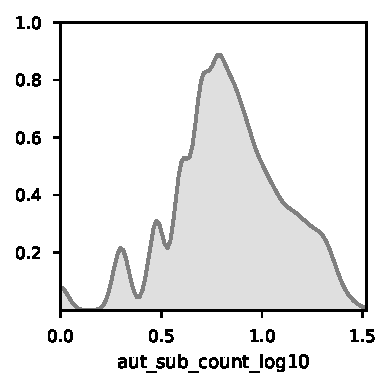
\includegraphics[width=\textwidth]{latex/kde/aut_sub_count_log10-active}
        \label{hist/aut:sub}
    \end{subfigure}
    \hfill
    \begin{subfigure}[b]{0.49\textwidth}
        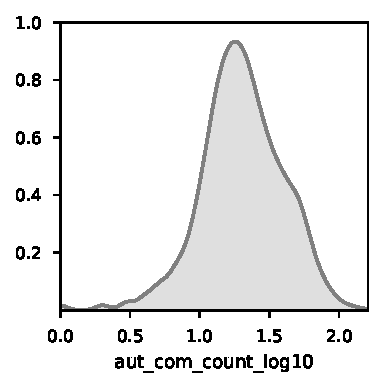
\includegraphics[width=\textwidth]{latex/kde/aut_com_count_log10-active.pdf}
        \label{hist/aut:com}
    \end{subfigure}
    \hfill
    \begin{subfigure}[b]{0.49\textwidth}
        \centering
        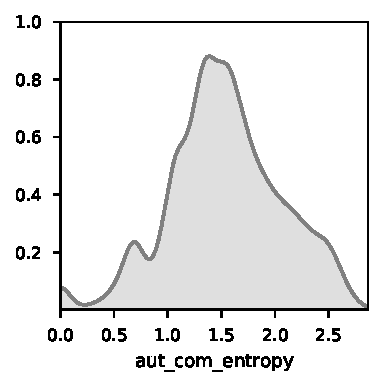
\includegraphics[width=\textwidth]{latex/kde/aut_com_entropy-active.pdf}
        \label{hist/aut:entropy}
    \end{subfigure}
    \hfill
    \begin{subfigure}[b]{0.49\textwidth}
        \centering
        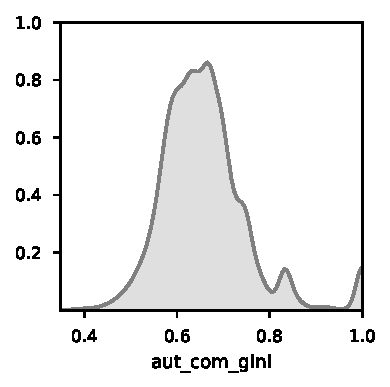
\includegraphics[width=\textwidth]{latex/kde/aut_com_gini-active.pdf}
        \label{hist/aut:gini}
    \end{subfigure}
    \hfill
    \begin{subfigure}[b]{0.49\textwidth}
        \centering
        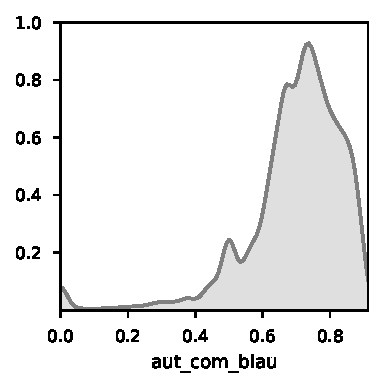
\includegraphics[width=\textwidth]{latex/kde/aut_com_blau-active.pdf}
        \label{hist/aut:blau}
    \end{subfigure}
    \hfill
    \begin{subfigure}[b]{0.49\textwidth}
        \centering
        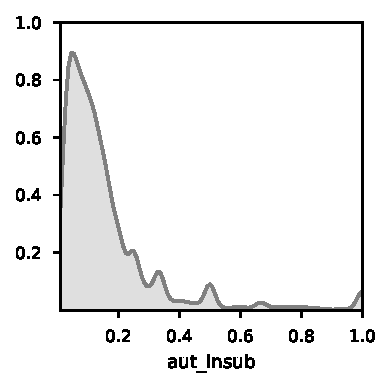
\includegraphics[width=\textwidth]{latex/kde/aut_insub-active.pdf}
        \label{hist/aut:insub}
    \end{subfigure}
    \caption{Distributions of Author-Level Statistics for Active Subreddits}
\end{figure} \label{hists/aut:active}

\subsection{General Trends}
Again focusing on active subreddits - what are the stats for these values of the author level?

Table \ref{table/author-medians:active} shows the descriptive statistics of the author-level measures for active subreddits. Figure \ref{hists/aut:active}


Table \ref{table/author-medians:all} shows the results for all subreddits. Again the count values are highly skewed across subreddits. The lower 75\% of subreddits have an average author subreddit count of 14.5 or less, and an average author comment count of 58 or less. However the maximum values are 7,996 and 1,245,236, respectively. 433 subreddits have these values because all were only commented in by 1 redditor, \textit{imguralbumbot}, a known bot account. Therefore, I again selected the top decile of subreddits by author count for further analysis.

Table \ref{table/author-medians:active} shows the results for the top decile of active subreddits. 
......

\begin{figure}
    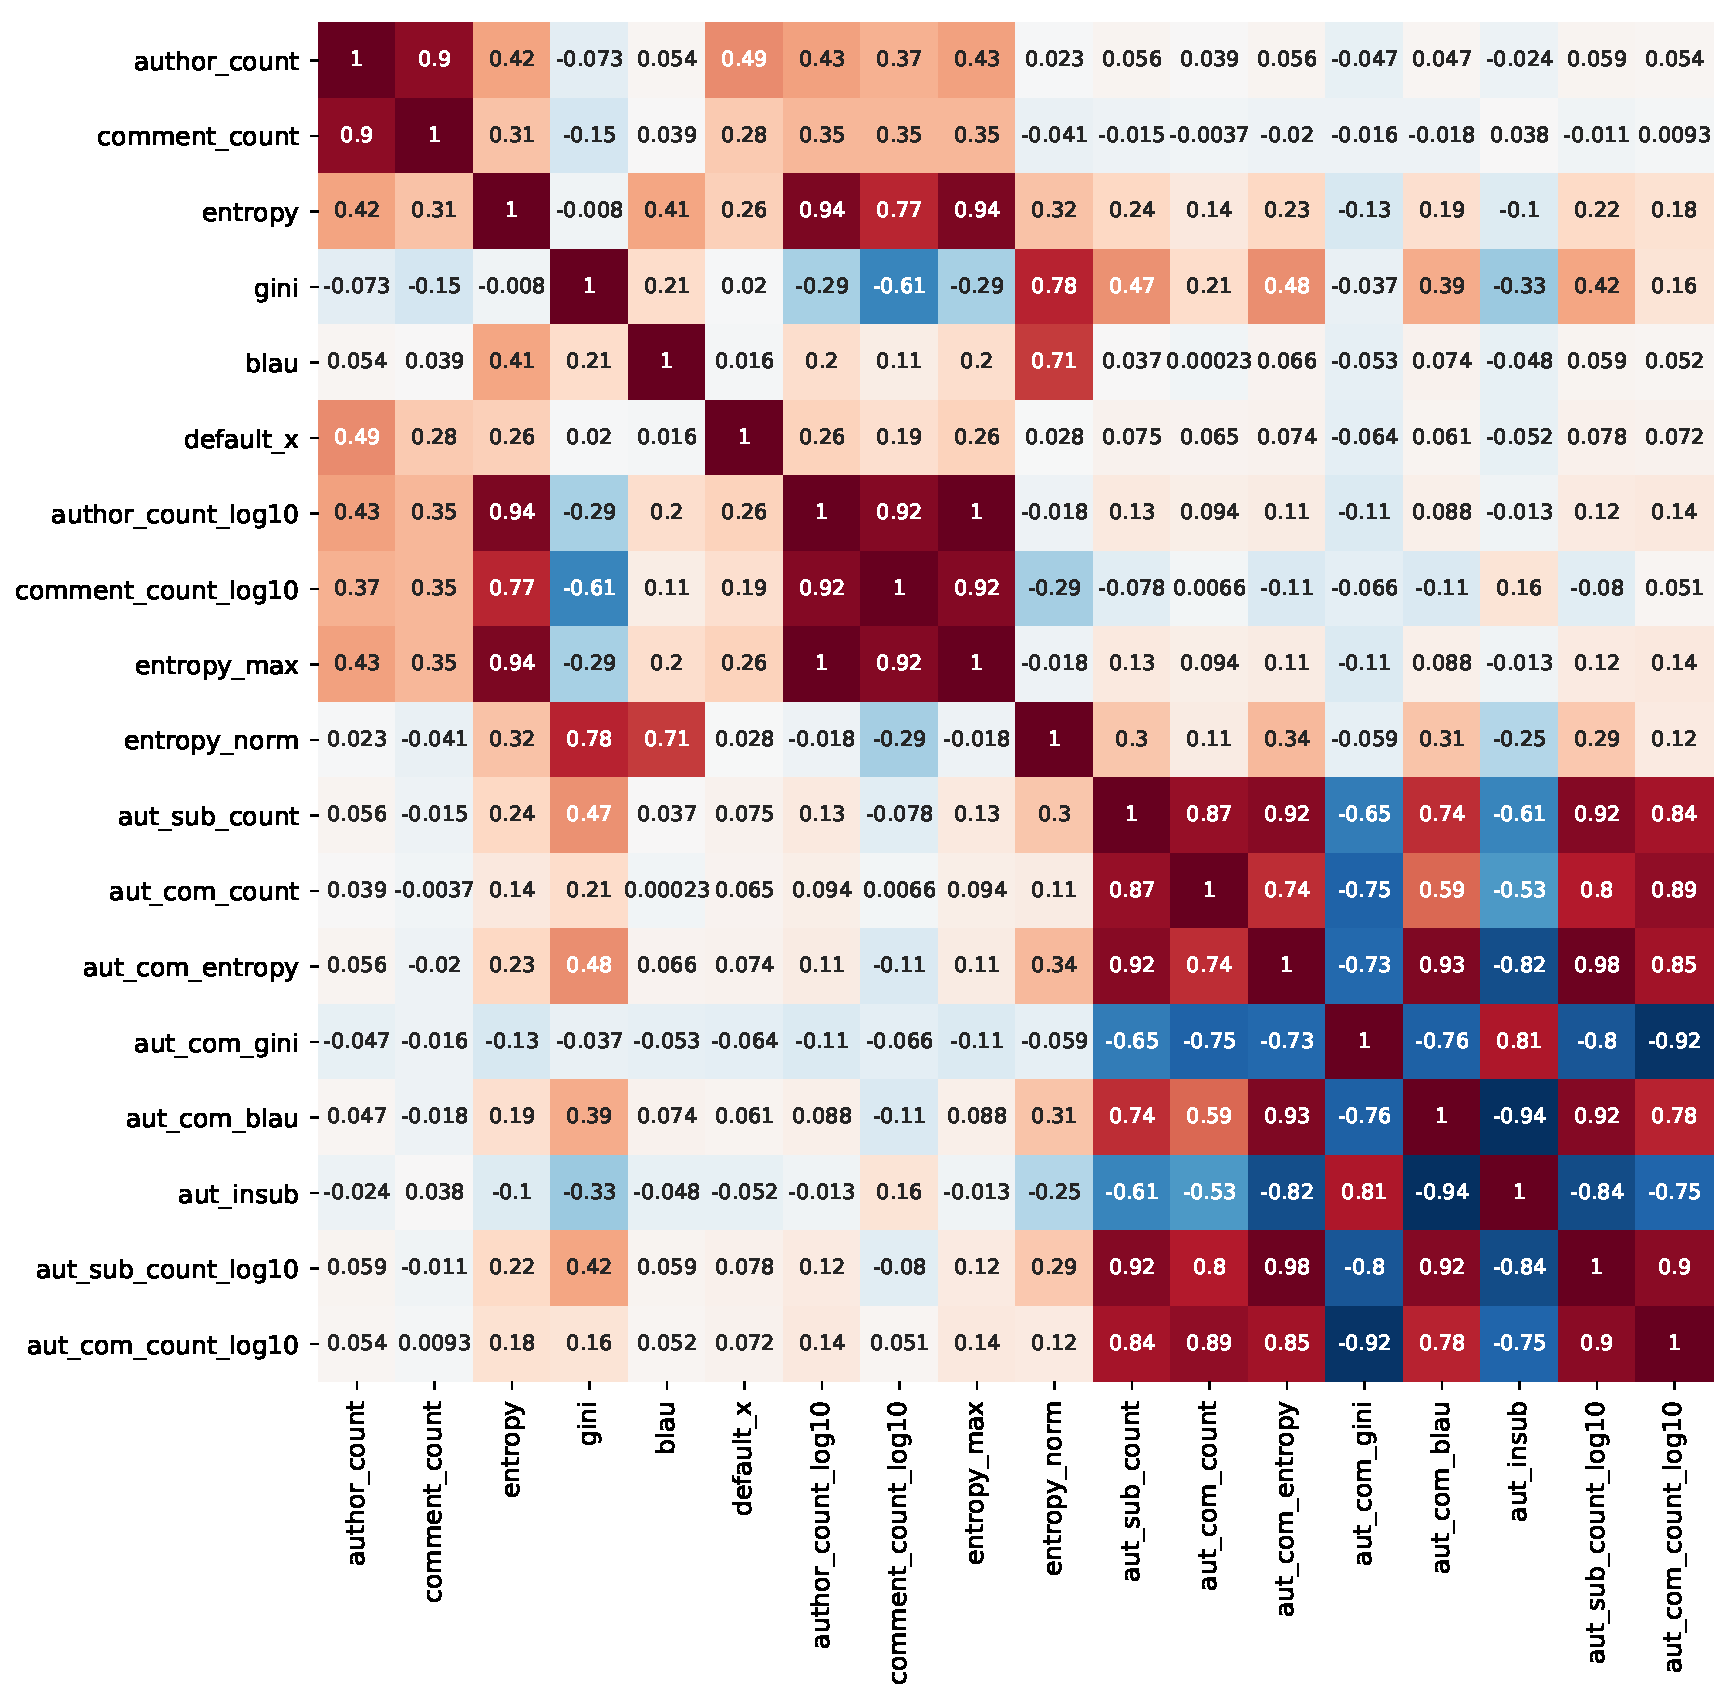
\includegraphics[scale=0.55]{latex/matrix/corr-heat-active.pdf}
    \caption{Correlation Heatmap of Subreddit- and Author-Level Statistics for Active Authors}
    \label{corr-heat}
\end{figure}

Figure \ref{corr-heat} shows the correlations among subreddit- and author-level statistics for active subreddits. The heat map is coloured from dark red (correlation = 1) to dark blue (correlation = -1). The paler the colour, the closer it is to 0. The pale upper-right and lower-left quadrants show that most subreddit-level statistics are not highly correlated, either positively or negatively) with author-level statistics for active subreddits. This is particularly important for author\_count and comment\_count: the author-level statistics are not dependent on subreddit size.

There subreddit-level statistics with some correlation with author-level statistics are entropy, blau, and normalised entropy.

\textcolor{red}{Get separate clustermap for author-level statistics. Most square are dark red or dark blue, how do they cluster?}


\begin{figure}
    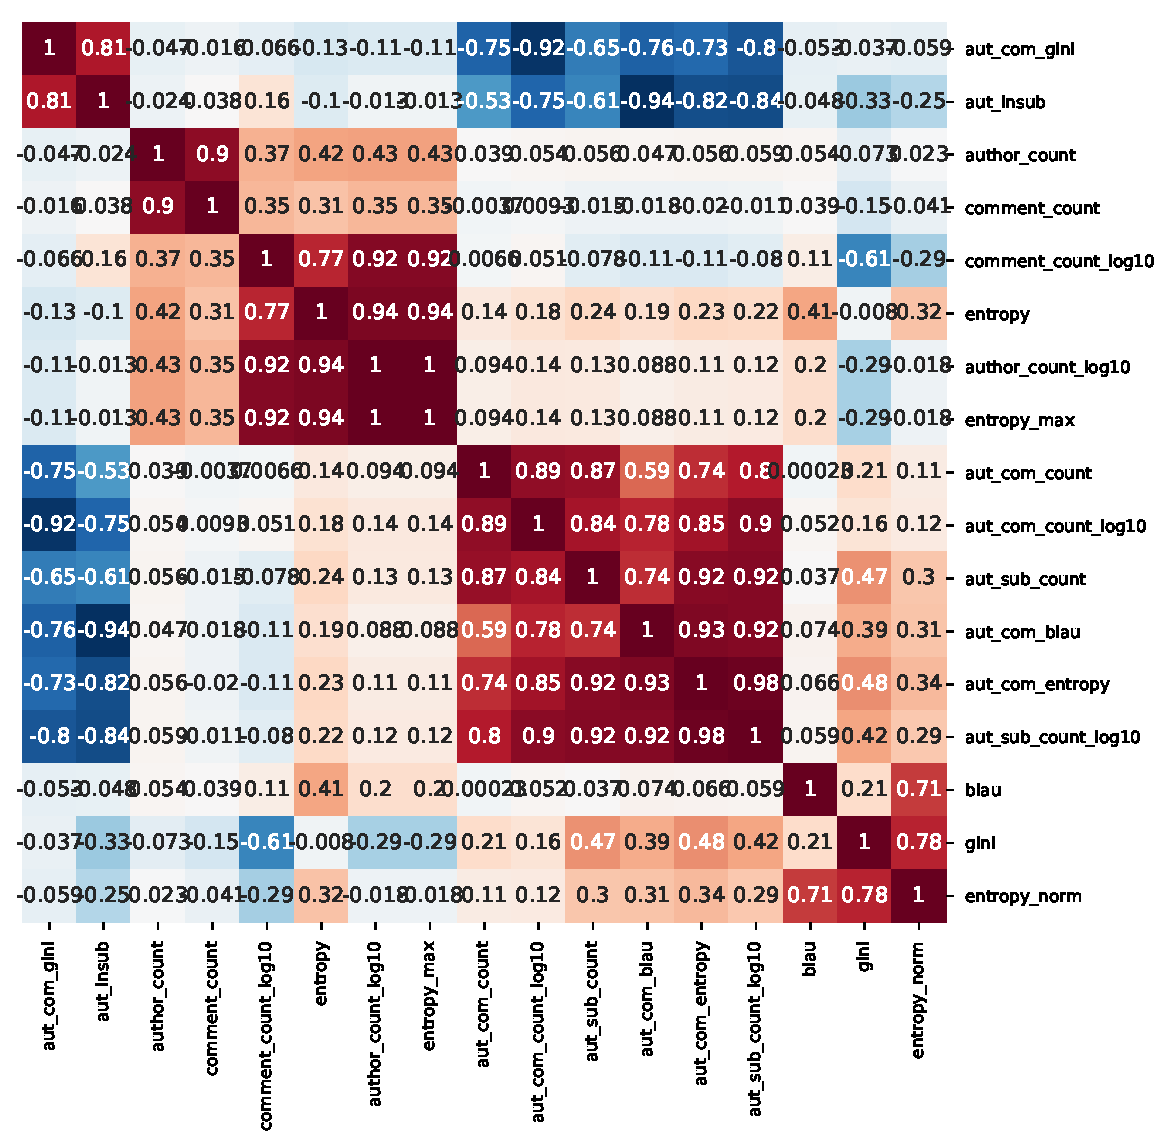
\includegraphics[scale=0.8]{latex/matrix/corr-cluster-active.pdf}
    \caption{Correlation Clustermap of Subreddit- and Author-Level Statistics for Active Authors}
    \label{corr-cluster}
\end{figure}
